\subsection{Sequence Diagram}

Figure 1 illustrates the sequence diagram depicting the process of user registration. It begins with the user initiating a post request to the SignUpServlet. The SignUpServlet then forwards the email validation request to Utils, followed by a query to UserDAO searching for existing users with the provided email. If no user matches the email, SignUpServlet proceeds by sending a request to add a new user to the UserDAO. 

\begin{figure}[h]
    \centering
    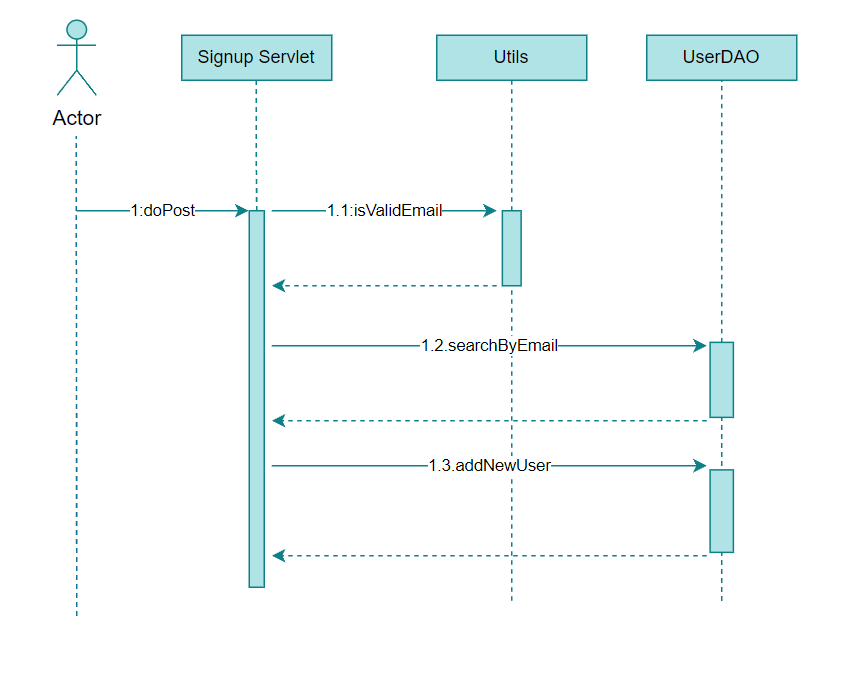
\includegraphics[width=0.75\linewidth]{sections/BLL/SignUpSqDiag.png}
    \caption{Sequence Diagram for User Sign Up}
    \label{fig:sequence-diagram-signup}
\end{figure}

The figure 2 represents the sequence diagram for the operation actor login. The Actor, acting as the primary initiator, triggers the login process by submitting a "doPost" request to the Login Servlet. Subsequently, upon receiving this request, the Login Servlet proceeds by dispatching a "Login" request to the Session Manager. In turn, the Session Manager, acting as an intermediary, relays this request to the User Data Access Object (UserDAO) as a "verifyCredentials" operation. Following authentication of the user's credentials, UserDAO promptly returns a response to the Session Manager, which in turn communicates the outcome back to the Login Servlet, thus completing the login sequence.

\begin{figure}[h]
    \centering
    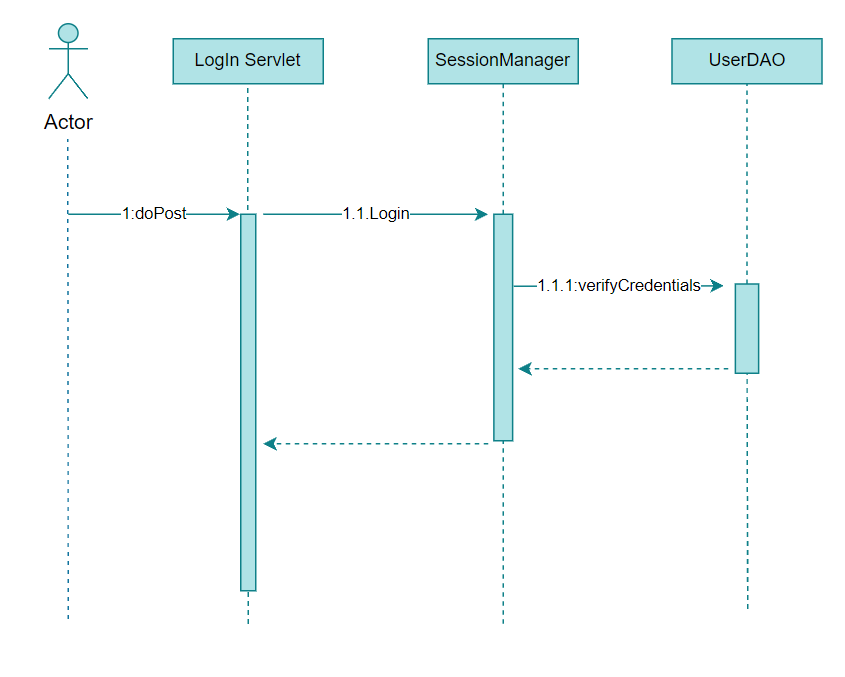
\includegraphics[width=0.75\linewidth]{sections/BLL/LoginSqDiag.png}
    \caption{Sequence Diagram for Actor Login}
    \label{fig:sequence-diagram-login}
\end{figure}



